\chapter{State of the art}\label{SotA}

Tady:

- Motion planning as a whole, tj.\ začít s 2D robotem a vysvětlit obecné koncepty, abych se k tomu mohl vracet -- grafové algoritmy, APF, RRT.

- Generalizace A*, APF a RRT na robotická ramena, reference na aktuální články.

- Metody specifické pro robotická ramena, tj.\ hlavně optimalizační.

- Existující pokusy zkombinovat IK a motion planning, tj.\ podobné tomu co dělám já.

Before we get into the problem of motion planning for robotic manipulators, let us take a step back and look at motion planning as a whole. This is arguably the most researched problem in robotics; there have been thousands of research papers with the motion planning keyword published in the recent years~\cite{RASreview}. The motion planning problem goes beyond a specific type of robot, or a specific problem; the term encapsulates movement of a robotic arm, legged robots, autonomous cars and even devices for exploration of oceans and space.
As researchers try to develop new algorithms and push the boundaries of what is computable, there are a few concepts at the core of each method, which are worth taking a look at.

\section{General concepts -- path planning for a 2D robot}

\begin{wrapfigure}{r}{0.33\textwidth}
    \centering
    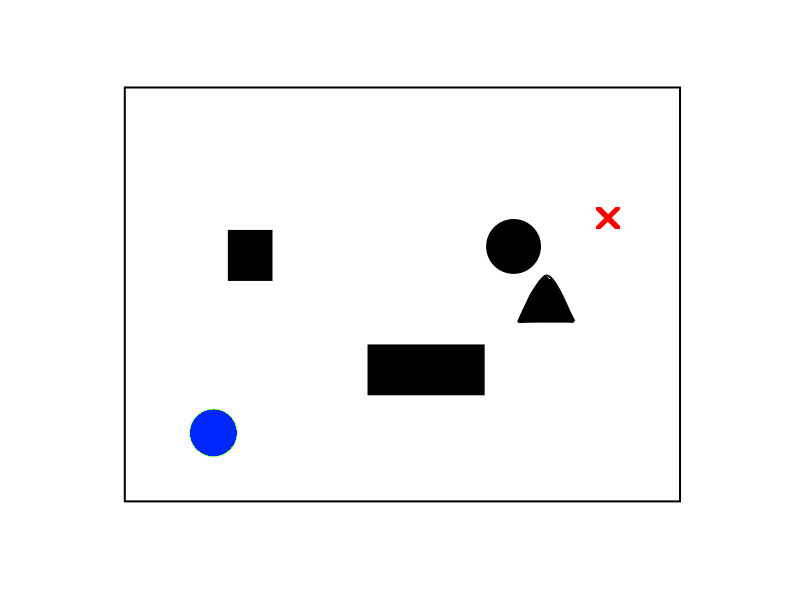
\includegraphics[width=0.32\textwidth]{robot_obstacles.png}
  \caption{A moving robot (blue) in 2 dimensions, trying to reach a target (red) while avoiding obstacles (black).}\label{fig:bot}
\end{wrapfigure}

For simplicity, let us consider the case of a robot that can move in any direction, trying to find a path to a goal in a 2-dimensional space with some obstacles. We refer to this problem as path planning; since we are only concerned with finding a path and not realising the actual movement, it is a subproblem of motion planning, though the terms are sometimes used interchangeably.

We will assume that the robot has full knowledge of the environment, and the environment remains unchanging. This is a heavy simplification, as real robots generally have limited ways of movement, and real life environments can often change dynamically. However, this simplified representation will let us easily visualize and understand each of the concepts before discussing their extensions. Later on, we shall take a look at how the algorithms can be generalised to higher dimensions and applied to robotic manipulators specifically.

The first idea that comes to mind after completing a basic algorithms course is to use algorithms for finding the shortest paths, such as the asymptotically optimal Djisktra's algorithm. The problem is that the space we are moving in is continuous, while the shortest path graph algorithms require discrete graphs connected with edges.

\begin{wrapfigure}{r}{0.33\textwidth}
    \centering
    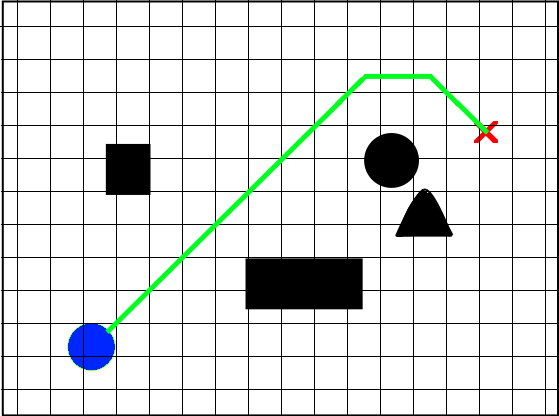
\includegraphics[width=0.32\textwidth]{robot_grid_path.png}
  \caption{\\Path to target found by Djikstra's algorithm on a grid.}\label{fig:grid}
\end{wrapfigure}

An intuitive approach to discretizing our space is creating a grid that represents the space, treating the points on the grid as vertices, and assigning the edges that lead to an occupied square an infinite cost. On this grid, finding the shortest path is a simple task. The main advantages to such an approach are implementational simplicity and easy generalization to 3 dimensions. Further constraints can be implemented using the weights on the grid; for example, when planning the path for a car, the weight on edges can reflect the speed limit on the corresponding road.
This method has been used successfully as a base for motion planning of autonomous vehicles~\cite{grid1, grid2}.

The main problem is choosing the size and shape of the grid. If the spacing between the vertices is too large, the resulting path diverges further from the optimal one, and the algorithm might not find a valid solution in a space with many small obstacles. However, if the spacing is too small, the number of vertices that need to be explored can easily become too large to compute in a reasonable amount of time.


\begin{wrapfigure}{r}{0.33\textwidth}
    \centering
    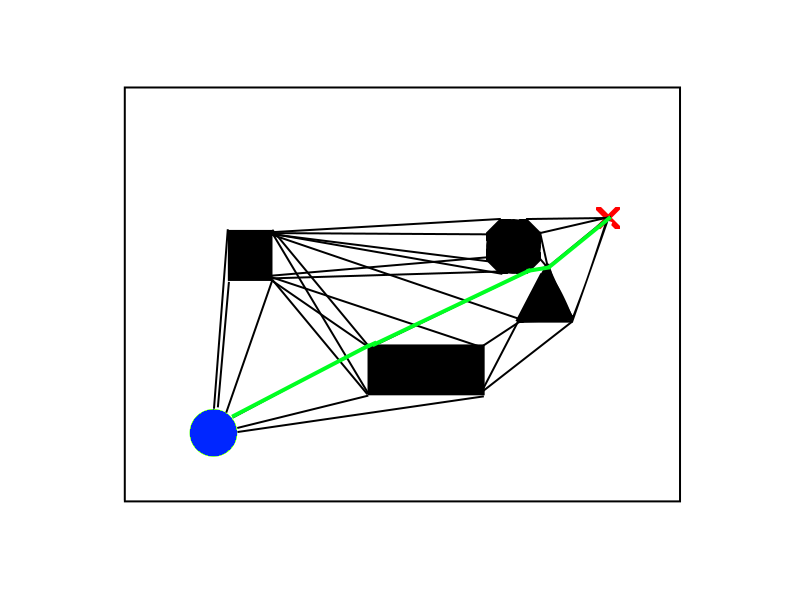
\includegraphics[width=0.32\textwidth]{robot_visibility.png}
  \caption{\\Shortest path on a visibility graph.}\label{fig:vis}
\end{wrapfigure}

In an effort to reduce the size of our graph and thereby speed up the graph-based path planning methods, visibility graphs have been suggested. To construct a visibility graph, obstacles in the workspace need to be approximated with polygons of choice. The corners of these polygons become the vertices of our graph. Two vertices are connected with an edge if they see each other in the intuitive sense: there is no obstacle on the direct line between them. Each edge is assigned weight corresponding to the euclidean distance of the vertices. Then, standard shortest path algorithms are computed on the graph.

\begin{wrapfigure}{l}{0.33\textwidth}
    \centering
    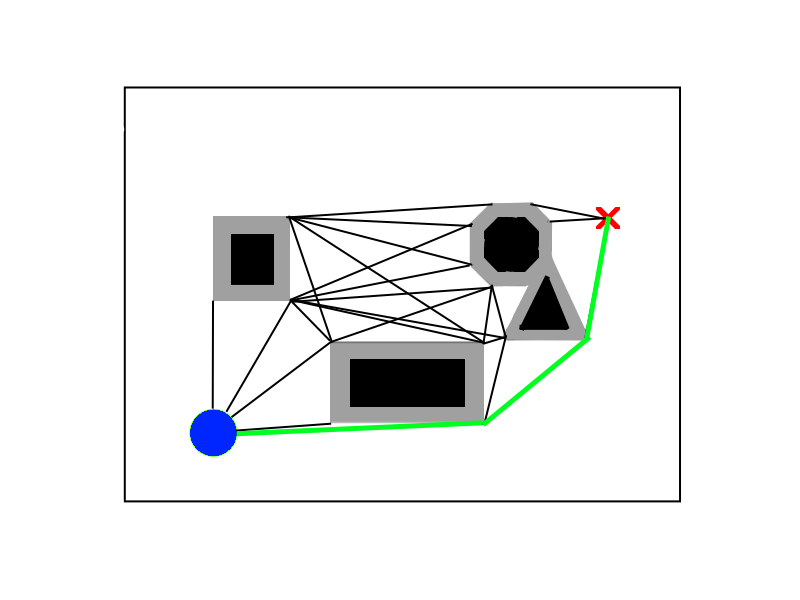
\includegraphics[width=0.32\textwidth]{robot_visibility_ext.png}
  \caption{\\Shortest path on a widened visibility graph.}\label{fig:vis_ext}
\end{wrapfigure}

As we can see in Figure~\ref{fig:vis}, the basic method can find impossible paths, since it does not account for the size of the robot. The way to mitigate this problem is to extend the size of each obstacle with respect the size and movement limitations of our robot; in the simplified problem, simply expanding each obstacle by the robot's radius is enough. The advantage to this approach is that we can reduce the size of the graph and still find an optimal path in the 2D path planning problem. A dynamic extension has also been suggested~\cite{DVG}, which makes the algorithm more flexible in changing environments.

Unfortunately, the method does not scale well to 3 dimensions, as the optimal path rarely leads directly around obstacles. We also need to be wary of imprecisions in the robot's movement; a path close to the obstacles could easily lead to a collision upon a mechanical error. These disadvantages have made the method less popular in recent years.

The opposite approach has been more successful. Rather than considering points as close to the obstacles as possible, we can consider the furthest points from nearby obstacles, and construct a so-called Voronoi diagram. This method provides safe and smooth paths for the robot~\cite{voronoi} and is still used today as a base for modern motion planning algorithms~\cite{voronoi2}. However, much like the previous method, voronoi diagrams are hard to scale to more than 2 dimensions. Therefore, they will not be as useful for our use case.

Regardless of the resulting shape of the graph, the choice of the shortest path algorithm can play a significant role in the path planning problem. Rather than using the traditional Djikstra's algorithm, the modern approach is to use the A* algorithm.

The A* algorithm~\cite{ai_modern} can be viewed as an extension of Djikstra's shortest path algorithms and uses a heuristic which influences what nodes will be chosen during the graph search. Under two conditions, the algorithm is complete\footnote{If a solution exists, the algorithm will find the best one.} and asymptotically optimal. The first condition on the heuristic is admissibility -- the heuristic never overestimates the cost to reach the goal. The second is consistency -- the value estimated by the heuristic is always less than or equal to the estimated distance from any neighbouring vertex to the goal, plus the cost of reaching that neighbour.

Since we are discussing the problem of finding a path to a target, a simple heuristic that is both admissible and consistent is the euclidean distance of a vertex to the target. Exploring vertices based on the distance from the target can often lead to obtaining a much faster solution, but gives us no guarantees on actually being faster than Djikstra.

The disadvantage to using this algorithm is that a suitable heuristic can be hard to find, and the worst case space complexity is higher than for Djikstra's algorithm. Still, the algorithm is widely used and and can be generalized to further problems.

\newpage
If we relax the requirement of finding an optimal solution and look for faster algorithms that provide \enquote{good enough} solutions, we can move away from graph-based approaches. Gradient based approaches make local decisions based on some criteria, and iteratively move towards the target. Among these, a path planning algorithm that stands out is the Artificial Potential Field (APF) method.

\begin{wrapfigure}{r}{0.33\textwidth}
    \centering
    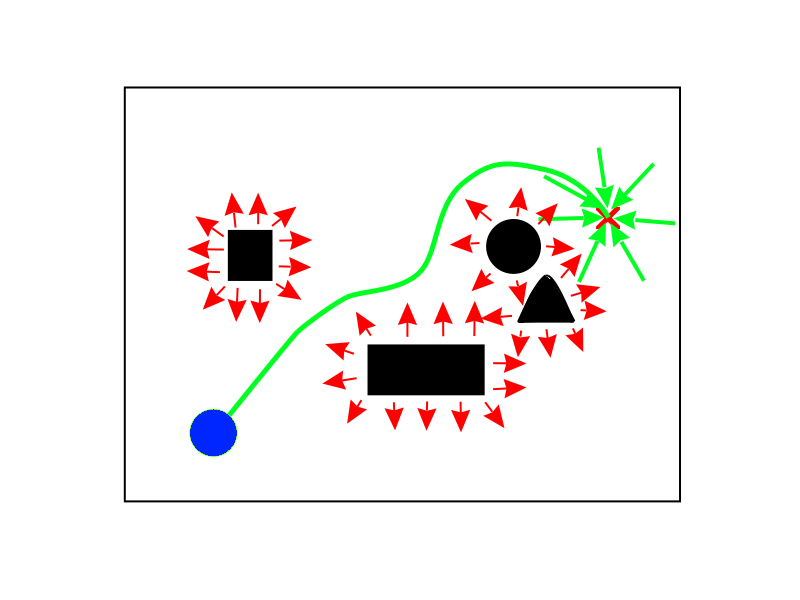
\includegraphics[width=0.32\textwidth]{robot_apf.png}
  \caption{\\Path found by the APF algorithm.}\label{fig:apf}
\end{wrapfigure}

Intuitively, objects in the APF algorithm act on our robot as magnets. The target attracts our robot with a strong force, while the obstacles repulse the robot. In an ideal scenario, this results in finding a smooth path to the target while avoiding obstacles. This algorithm is highly efficient, and can be extended to various problems. Besides its low cost, one of the main advantages is that the algorithm can quickly react to a changing environment, which makes it more flexible in dynamic environments compared to the graph-based methods.

\begin{wrapfigure}{l}{0.33\textwidth}
    \centering
    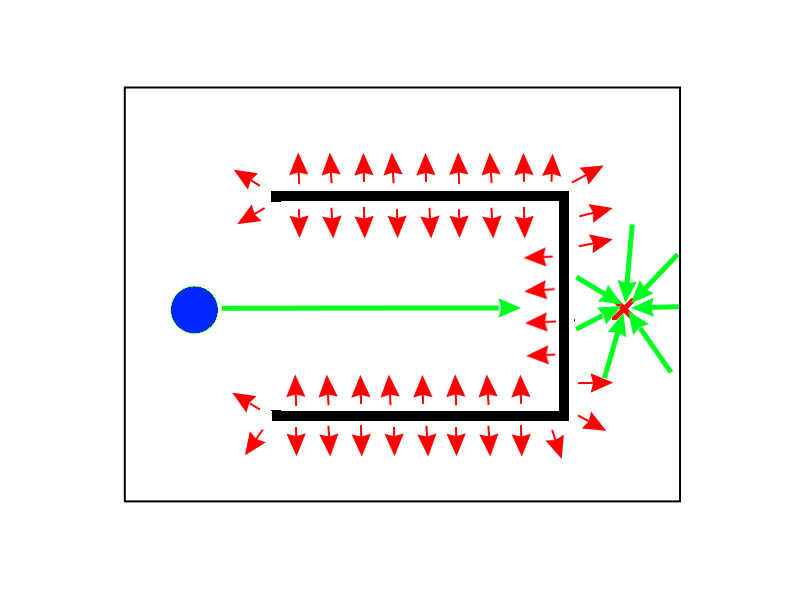
\includegraphics[width=0.32\textwidth]{robot_apf_min.png}
  \caption{\\Local minimum in APF algorithm.}\label{fig:apf_min}
\end{wrapfigure}

There are two main downsides to the algorithm. For one, it gives us no guarantees on the optimality of the found path; but even worse than that, the basic version is susceptible to local minima. Some authors suggest extensions that help the robot get around obstacles~\cite{apf, apf2}, while another common use for the algorithm is to plan a global path using a graph-based method and use APF to make local decisions and actually realise the movement~\cite{hybrid}. Since this method can easily be generalised to more dimensions, it will be of interest later on.

\newpage
The last family of algorithms is based on random sampling.
